\documentclass{beamer} 
\usepackage[utf8]{inputenc}
\usetheme{Frankfurt}  %% Themenwahl
\usecolortheme{whale}

\title{Markdown - eine kurze Vorstellung}
\author{Fnordberg}
\date{\today}
\titlegraphic{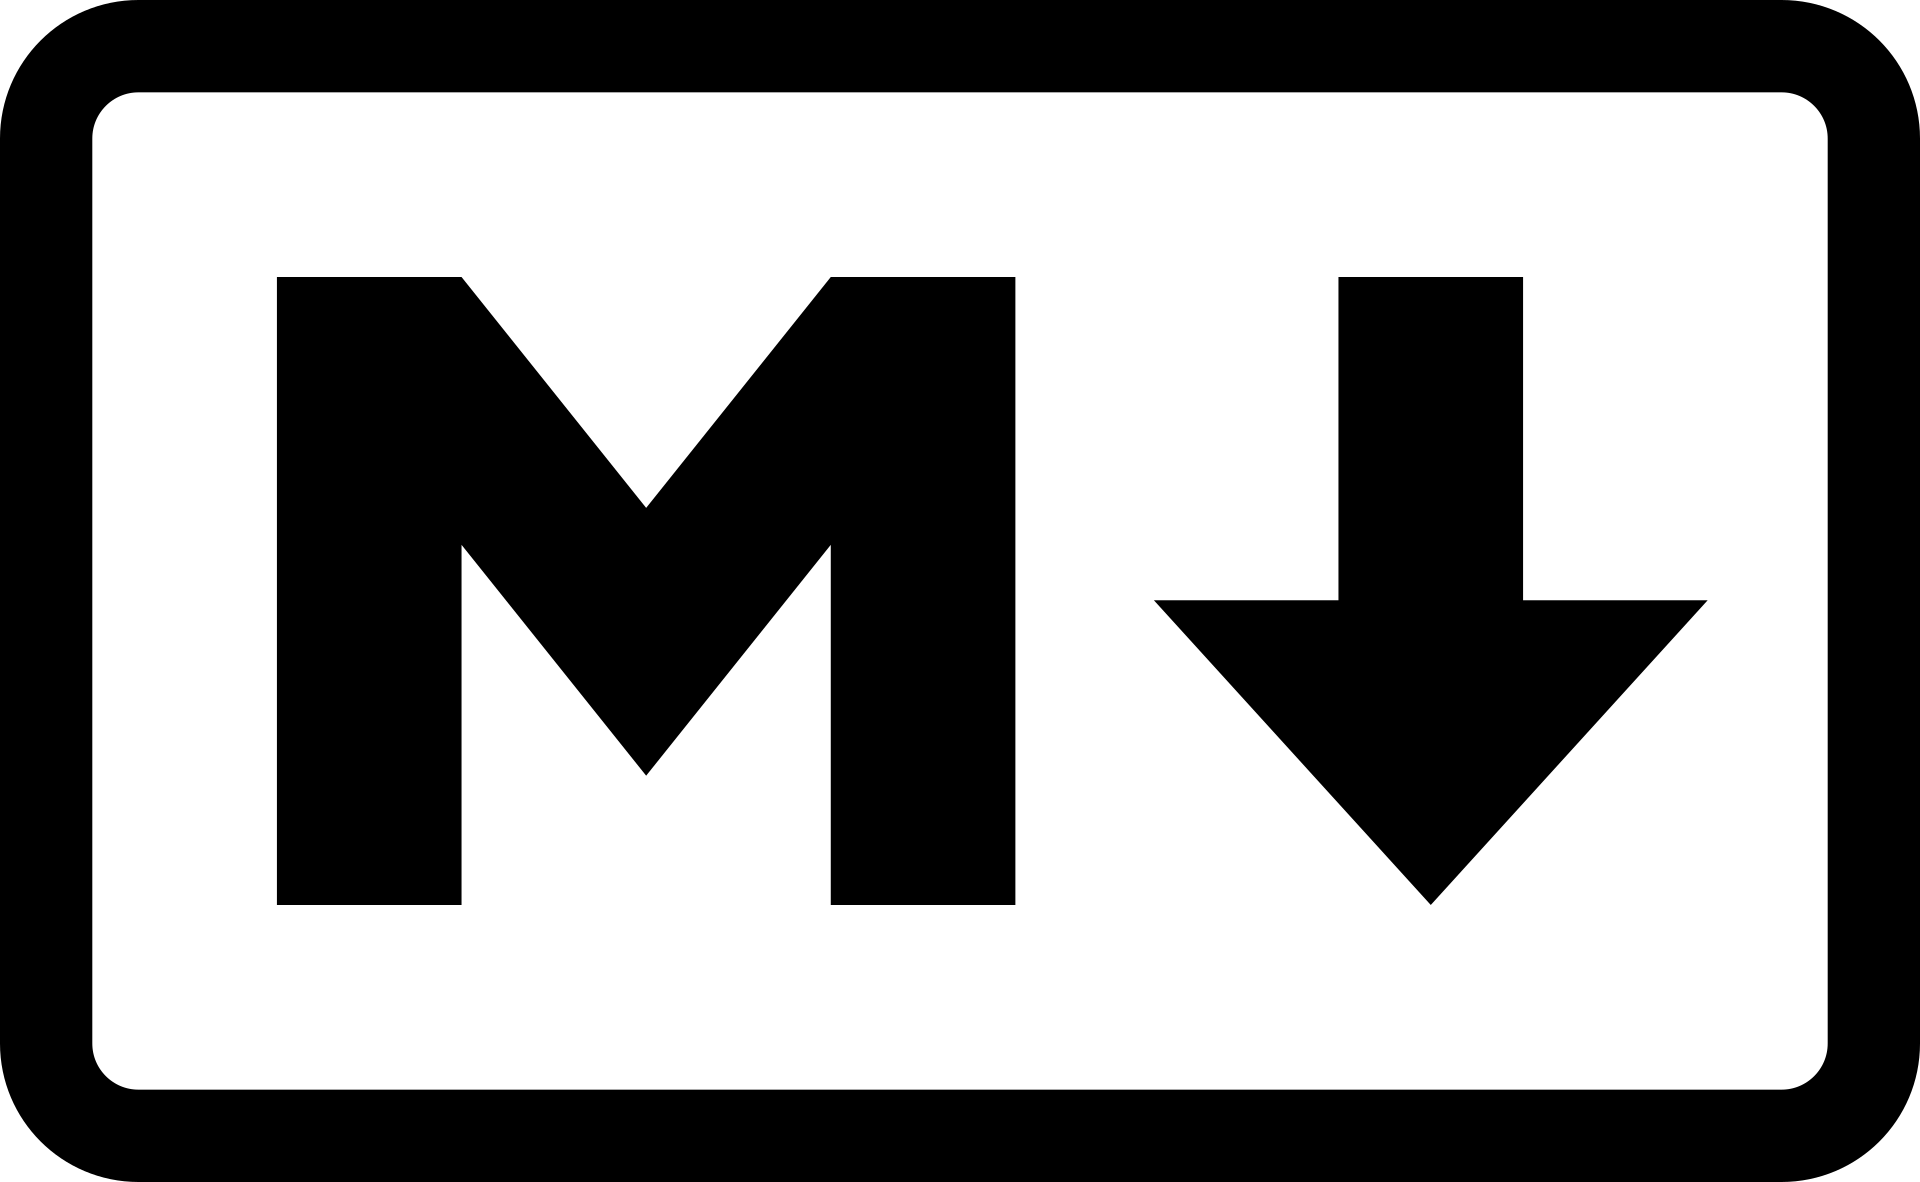
\includegraphics[scale=0.05]{markdown-logo.png}}

%Beginn

\begin{document}
\maketitle

\section{Was ist Markdown?}
\begin{frame}{Was möchte ich mit diesen Vortrag erreichen?}
    \begin{minipage}[b]{75mm}
        \begin{itemize}
            \item einen Einblick geben
            \item wichtige Anwendungsmöglichkeiten
            \item eine kleine Einführung in die Grundlegende Syntax geben
        \end{itemize}
    \end{minipage}
        \hfill
    \begin{minipage}[b]{25mm}
        
\includegraphics[width=25mm]{pic-tux_1.png}
    \end{minipage}
\end{frame}

\begin{frame}{Was möchte ich mit diesen Vortrag \textbf{nicht} erreichen?}
    \begin{minipage}[b]{75mm}
        \begin{itemize}
            \item keine Bekehrung
            \item keine Allumfassende Einführung geben
            \item euch langweilen
        \end{itemize}
    \end{minipage}
        \hfill
    \begin{minipage}[b]{25mm}
        
\includegraphics[width=25mm]{pic-tux_2.png}
    \end{minipage}
\end{frame}

%Allgemein

\begin{frame} 
  \frametitle{Markdown} 
    \begin{itemize}
        \item ist eine Aufzeichnungssprache (Markup language) ähnlich wie \LaTeX oder HTML
        \item wurde von John Grubber und Aron Swartz
        \item besitzt eine einfache Syntax
        \item ist einfach und schnell zu lernen
        \item ist einfach zu lesen auch ohne Konvertierung 
        \item besitzt die Endung \textbf{.md} oder \textbf{.markdown}
    \end{itemize}
\end{frame}

\section{Wo wird Markdown benuzt?}

% Github/Gitlab

\begin{frame}{Github/Gitlab}
        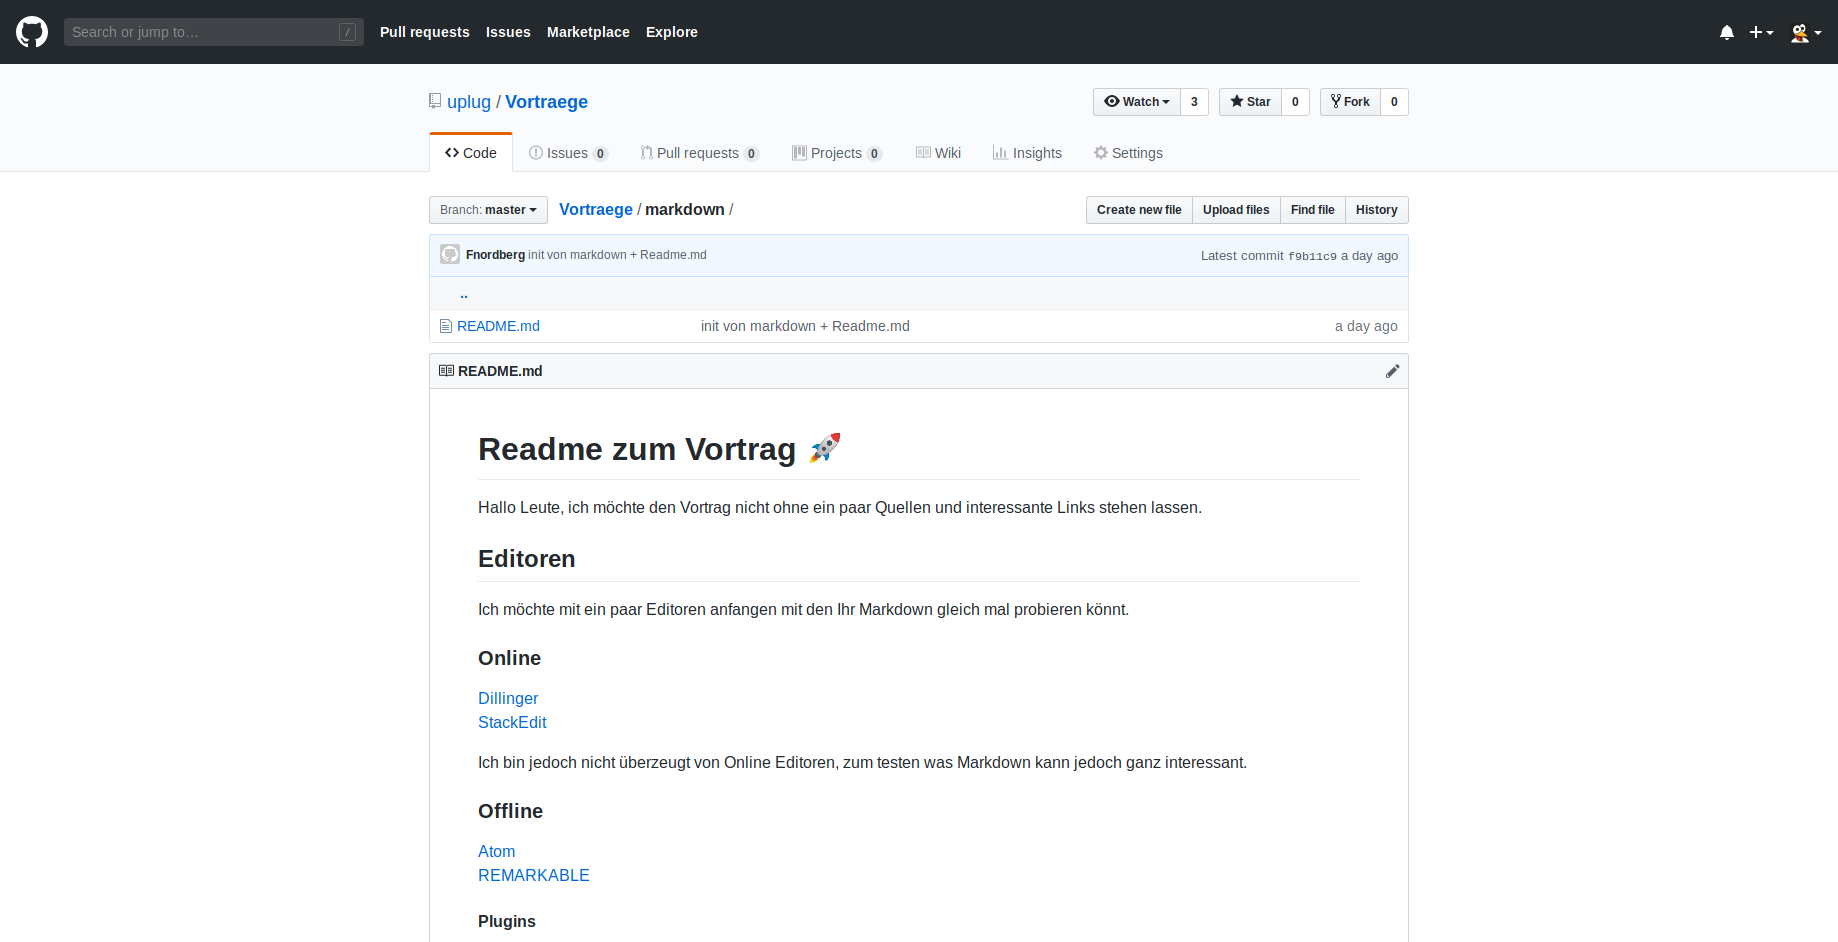
\includegraphics[scale=0.18]{github.png}
\end{frame}

% Stackoverflow

\begin{frame}{Stackoverflow}
        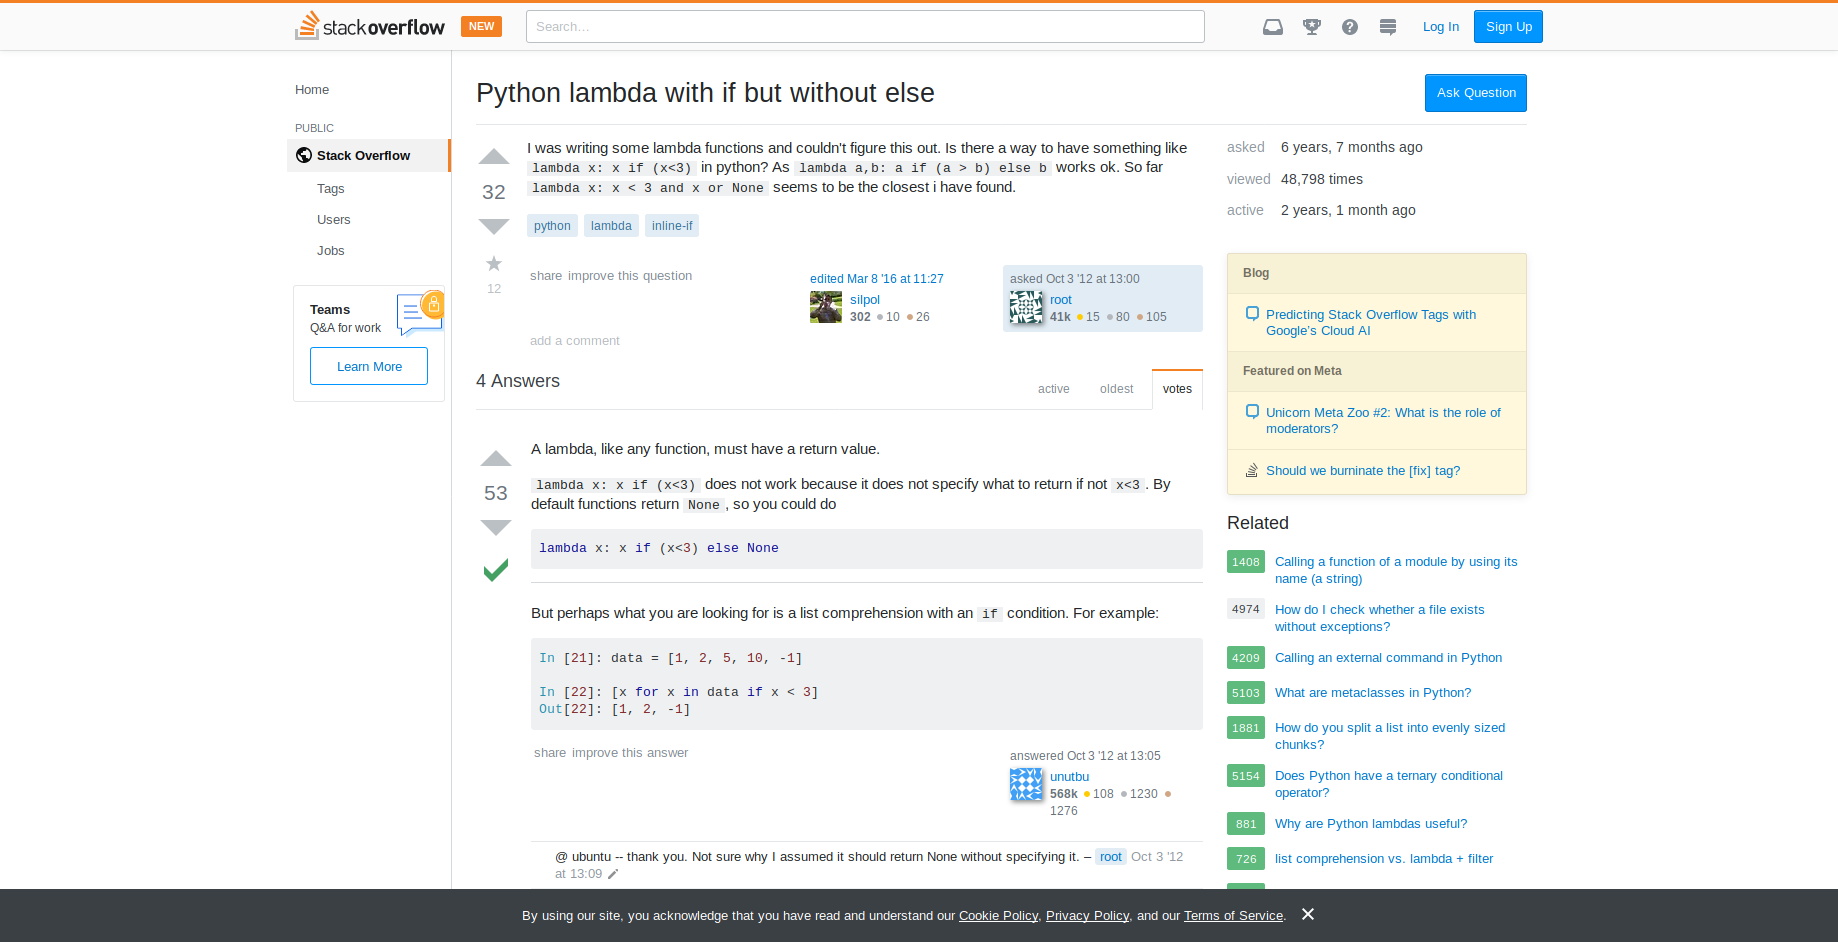
\includegraphics[scale=0.18]{stackoverflow.png}
\end{frame}

% persönliche Aufzeichnungen

\begin{frame}{Persönliche Aufzeichnungen}
        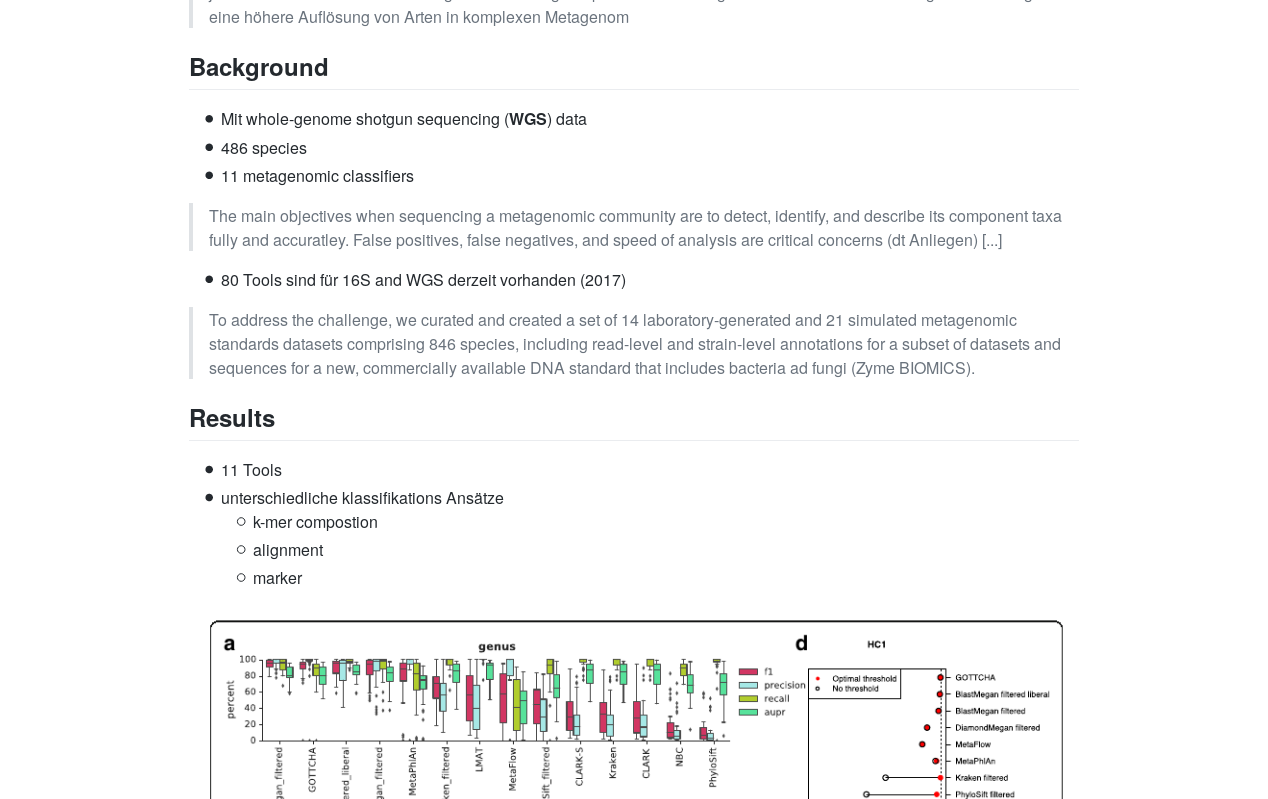
\includegraphics[scale=0.25]{aufzeichnungen.png}
\end{frame}

% Editoren

\section{Markdown Editoren}

\begin{frame}{Markdown - aber wie?}
\begin{itemize}
    \item klassische Editoren (die guten) mit Plugins
    \begin{itemize}
        \item Vim
        \item Emacs
    \end{itemize}
    \item neuere Editoren    
    \begin{itemize}
        \item Atom
        \item Juypter
        \item Sublime
    \end{itemize}
    \item Online Editoren
    \begin{itemize}
        \item Dillinger
    \end{itemize}
    \item Dokumenten Konverter
        \begin{itemize}
            \item Pandoc
        \end{itemize}
    \end{itemize}
\end{frame}

% Grundlagen

\section{Was kann Markdown?}

\begin{frame}{Was kann Markdown?}
    \begin{itemize}
        \item Überschriften verschiedener Ordnung
        \item Listen
        \item Bilder einfügen
        \item Links
        \item Zitate
        \item Inline-Code
        \item Code-Block
        \item ...
    \end{itemize}
\end{frame}

\begin{frame}{Was ist Markdown nicht?}
    \begin{itemize}
        \item der heilige Gral
        \item ein adequater Ersatz für \LaTeX
        \item immer einheitlich
        \begin{itemize}
            \item CommonMark
            \item Pandoc Markdown
            \item Github Markdown
            \item R-Markdown
            \item Stackoverflow Markdown
        \end{itemize}
    \end{itemize}
\end{frame}
  
% Fragen?  

\begin{frame}{Bevor es los geht...}
    
\includegraphics[scale=0.17]{questions.jpg}
\end{frame}

% Praxis Teil

\section{Ein bisschen Praxis! :)}

\begin{frame}{...und nun ein bisschen Praxis!}
	Jetzt kommt der Mitmachteil!
\end{frame}
    
\end{document}

